\documentclass{standalone}
\usepackage{tikz}
\usetikzlibrary{patterns, positioning}

\begin{document}
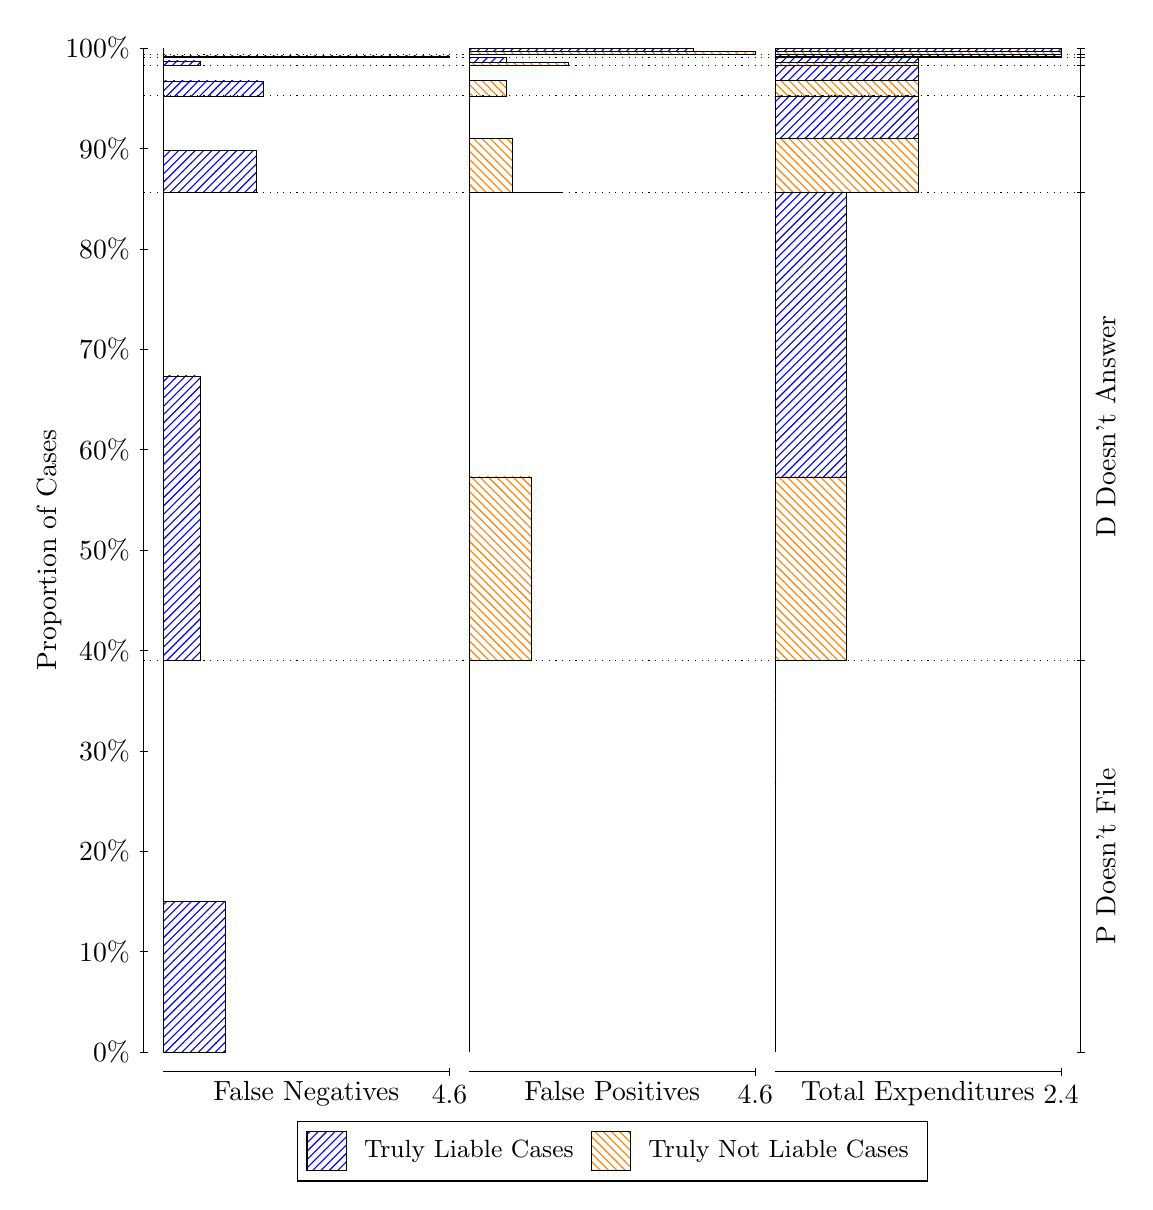
\begin{tikzpicture}
\draw[black, very thin] (1.5,1.75) -- (1.5,14.5);
\node[rotate=90, anchor=center] at (0.3, 8.125) {Proportion of Cases};
\draw[black, very thin] (1.45,1.75) -- (1.55,1.75);
\node[anchor=east] at (1.45, 1.75) {0\%};
\draw[black, very thin] (1.45,3.025) -- (1.55,3.025);
\node[anchor=east] at (1.45, 3.025) {10\%};
\draw[black, very thin] (1.45,4.3) -- (1.55,4.3);
\node[anchor=east] at (1.45, 4.3) {20\%};
\draw[black, very thin] (1.45,5.575) -- (1.55,5.575);
\node[anchor=east] at (1.45, 5.575) {30\%};
\draw[black, very thin] (1.45,6.85) -- (1.55,6.85);
\node[anchor=east] at (1.45, 6.85) {40\%};
\draw[black, very thin] (1.45,8.125) -- (1.55,8.125);
\node[anchor=east] at (1.45, 8.125) {50\%};
\draw[black, very thin] (1.45,9.4) -- (1.55,9.4);
\node[anchor=east] at (1.45, 9.4) {60\%};
\draw[black, very thin] (1.45,10.675) -- (1.55,10.675);
\node[anchor=east] at (1.45, 10.675) {70\%};
\draw[black, very thin] (1.45,11.95) -- (1.55,11.95);
\node[anchor=east] at (1.45, 11.95) {80\%};
\draw[black, very thin] (1.45,13.225) -- (1.55,13.225);
\node[anchor=east] at (1.45, 13.225) {90\%};
\draw[black, very thin] (1.45,14.5) -- (1.55,14.5);
\node[anchor=east] at (1.45, 14.5) {100\%};

\draw[black, very thin] (13.4,1.75) -- (13.4,14.5);
\draw[black, very thin] (13.35,1.75) -- (13.45,1.75);
\node[anchor=west] at (13.35, 1.75) {};
\draw[black, very thin] (13.35,6.7219) -- (13.45,6.7219);
\node[anchor=west] at (13.35, 6.7219) {};
\draw[black, very thin] (13.35,12.666) -- (13.45,12.666);
\node[anchor=west] at (13.35, 12.666) {};
\draw[black, very thin] (13.35,13.893) -- (13.45,13.893);
\node[anchor=west] at (13.35, 13.893) {};
\draw[black, very thin] (13.35,14.277) -- (13.45,14.277);
\node[anchor=west] at (13.35, 14.277) {};
\draw[black, very thin] (13.35,14.378) -- (13.45,14.378);
\node[anchor=west] at (13.35, 14.378) {};
\draw[black, very thin] (13.35,14.421) -- (13.45,14.421);
\node[anchor=west] at (13.35, 14.421) {};
\draw[black, very thin] (13.35,14.5) -- (13.45,14.5);
\node[anchor=west] at (13.35, 14.5) {};

\draw[black, very thin, pattern color=blue, pattern=north east lines] (1.75,1.75) rectangle (2.5399,3.6597);
\draw[black, very thin, pattern color=orange, pattern=north west lines] (1.75,3.6597) rectangle (1.75,6.7219);
\draw[black, very thin, pattern color=blue, pattern=north east lines] (1.75,6.7219) rectangle (2.2239,10.335);
\draw[black, very thin, pattern color=orange, pattern=north west lines] (1.75,10.335) rectangle (1.75,12.666);
\draw[black, very thin, pattern color=blue, pattern=north east lines] (1.75,12.666) rectangle (2.9348,13.202);
\draw[black, very thin, pattern color=blue, pattern=north east lines] (1.75,13.202) rectangle (2.8558,13.202);
\draw[black, very thin, pattern color=blue, pattern=north east lines] (1.75,13.202) rectangle (2.7768,13.202);
\draw[black, very thin, pattern color=blue, pattern=north east lines] (1.75,13.202) rectangle (2.6978,13.202);
\draw[black, very thin, pattern color=blue, pattern=north east lines] (1.75,13.202) rectangle (2.6188,13.202);
\draw[black, very thin, pattern color=blue, pattern=north east lines] (1.75,13.202) rectangle (2.5399,13.202);
\draw[black, very thin, pattern color=blue, pattern=north east lines] (1.75,13.202) rectangle (2.4609,13.202);
\draw[black, very thin, pattern color=blue, pattern=north east lines] (1.75,13.202) rectangle (2.3819,13.202);
\draw[black, very thin, pattern color=blue, pattern=north east lines] (1.75,13.202) rectangle (2.3029,13.202);
\draw[black, very thin, pattern color=orange, pattern=north west lines] (1.75,13.202) rectangle (1.75,13.893);
\draw[black, very thin, pattern color=blue, pattern=north east lines] (1.75,13.893) rectangle (3.0138,14.083);
\draw[black, very thin, pattern color=orange, pattern=north west lines] (1.75,14.083) rectangle (1.75,14.277);
\draw[black, very thin, pattern color=blue, pattern=north east lines] (1.75,14.277) rectangle (2.2239,14.337);
\draw[black, very thin, pattern color=orange, pattern=north west lines] (1.75,14.337) rectangle (1.75,14.378);
\draw[black, very thin, pattern color=blue, pattern=north east lines] (1.75,14.378) rectangle (5.3833,14.4);
\draw[black, very thin, pattern color=orange, pattern=north west lines] (1.75,14.4) rectangle (1.75,14.421);
\draw[black, very thin, pattern color=orange, pattern=north west lines] (1.75,14.421) rectangle (1.75,14.455);
\draw[black, very thin, pattern color=blue, pattern=north east lines] (1.75,14.455) rectangle (1.75,14.5);
\draw[black, very thin, pattern color=orange, pattern=north west lines] (5.6333,1.75) rectangle (5.6333,4.8121);
\draw[black, very thin, pattern color=blue, pattern=north east lines] (5.6333,4.8121) rectangle (5.6333,6.7219);
\draw[black, very thin, pattern color=orange, pattern=north west lines] (5.6333,6.7219) rectangle (6.4232,9.0527);
\draw[black, very thin, pattern color=blue, pattern=north east lines] (5.6333,9.0527) rectangle (5.6333,12.666);
\draw[black, very thin, pattern color=orange, pattern=north west lines] (5.6333,12.666) rectangle (6.8181,12.666);
\draw[black, very thin, pattern color=orange, pattern=north west lines] (5.6333,12.666) rectangle (6.7391,12.666);
\draw[black, very thin, pattern color=orange, pattern=north west lines] (5.6333,12.666) rectangle (6.6601,12.666);
\draw[black, very thin, pattern color=orange, pattern=north west lines] (5.6333,12.666) rectangle (6.5812,12.666);
\draw[black, very thin, pattern color=orange, pattern=north west lines] (5.6333,12.666) rectangle (6.5022,12.666);
\draw[black, very thin, pattern color=orange, pattern=north west lines] (5.6333,12.666) rectangle (6.4232,12.666);
\draw[black, very thin, pattern color=orange, pattern=north west lines] (5.6333,12.666) rectangle (6.3442,12.666);
\draw[black, very thin, pattern color=orange, pattern=north west lines] (5.6333,12.666) rectangle (6.2652,12.666);
\draw[black, very thin, pattern color=orange, pattern=north west lines] (5.6333,12.666) rectangle (6.1862,13.356);
\draw[black, very thin, pattern color=blue, pattern=north east lines] (5.6333,13.356) rectangle (6.0283,13.356);
\draw[black, very thin, pattern color=blue, pattern=north east lines] (5.6333,13.356) rectangle (5.9493,13.356);
\draw[black, very thin, pattern color=blue, pattern=north east lines] (5.6333,13.356) rectangle (5.8703,13.356);
\draw[black, very thin, pattern color=blue, pattern=north east lines] (5.6333,13.356) rectangle (5.7913,13.356);
\draw[black, very thin, pattern color=blue, pattern=north east lines] (5.6333,13.356) rectangle (5.7123,13.356);
\draw[black, very thin, pattern color=blue, pattern=north east lines] (5.6333,13.356) rectangle (5.6333,13.893);
\draw[black, very thin, pattern color=orange, pattern=north west lines] (5.6333,13.893) rectangle (6.1072,14.087);
\draw[black, very thin, pattern color=blue, pattern=north east lines] (5.6333,14.087) rectangle (5.6333,14.277);
\draw[black, very thin, pattern color=orange, pattern=north west lines] (5.6333,14.277) rectangle (6.8971,14.319);
\draw[black, very thin, pattern color=blue, pattern=north east lines] (5.6333,14.319) rectangle (6.1072,14.378);
\draw[black, very thin, pattern color=orange, pattern=north west lines] (5.6333,14.378) rectangle (5.6333,14.4);
\draw[black, very thin, pattern color=blue, pattern=north east lines] (5.6333,14.4) rectangle (5.6333,14.421);
\draw[black, very thin, pattern color=orange, pattern=north west lines] (5.6333,14.421) rectangle (9.2667,14.455);
\draw[black, very thin, pattern color=blue, pattern=north east lines] (5.6333,14.455) rectangle (8.4768,14.5);
\draw[black, very thin, pattern color=orange, pattern=north west lines] (9.5167,1.75) rectangle (9.5167,4.8121);
\draw[black, very thin, pattern color=blue, pattern=north east lines] (9.5167,4.8121) rectangle (9.5167,6.7219);
\draw[black, very thin, pattern color=orange, pattern=north west lines] (9.5167,6.7219) rectangle (10.425,9.0527);
\draw[black, very thin, pattern color=blue, pattern=north east lines] (9.5167,9.0527) rectangle (10.425,12.666);
\draw[black, very thin, pattern color=orange, pattern=north west lines] (9.5167,12.666) rectangle (11.333,12.666);
\draw[black, very thin, pattern color=blue, pattern=north east lines] (9.5167,12.666) rectangle (11.333,12.666);
\draw[black, very thin, pattern color=orange, pattern=north west lines] (9.5167,12.666) rectangle (11.333,13.356);
\draw[black, very thin, pattern color=blue, pattern=north east lines] (9.5167,13.356) rectangle (11.333,13.893);
\draw[black, very thin, pattern color=orange, pattern=north west lines] (9.5167,13.893) rectangle (11.333,13.893);
\draw[black, very thin, pattern color=blue, pattern=north east lines] (9.5167,13.893) rectangle (11.333,13.893);
\draw[black, very thin, pattern color=orange, pattern=north west lines] (9.5167,13.893) rectangle (11.333,14.087);
\draw[black, very thin, pattern color=blue, pattern=north east lines] (9.5167,14.087) rectangle (11.333,14.277);
\draw[black, very thin, pattern color=orange, pattern=north west lines] (9.5167,14.277) rectangle (11.333,14.319);
\draw[black, very thin, pattern color=blue, pattern=north east lines] (9.5167,14.319) rectangle (11.333,14.378);
\draw[black, very thin, pattern color=orange, pattern=north west lines] (9.5167,14.378) rectangle (13.15,14.4);
\draw[black, very thin, pattern color=blue, pattern=north east lines] (9.5167,14.4) rectangle (13.15,14.421);
\draw[black, very thin, pattern color=orange, pattern=north west lines] (9.5167,14.421) rectangle (13.15,14.455);
\draw[black, very thin, pattern color=blue, pattern=north east lines] (9.5167,14.455) rectangle (13.15,14.5);
\draw[black, dotted] (1.5,6.7219) -- (13.4,6.7219);
\draw[black, dotted] (1.5,12.666) -- (13.4,12.666);
\draw[black, dotted] (1.5,13.893) -- (13.4,13.893);
\draw[black, dotted] (1.5,14.277) -- (13.4,14.277);
\draw[black, dotted] (1.5,14.378) -- (13.4,14.378);
\draw[black, dotted] (1.5,14.421) -- (13.4,14.421);
\draw[black, very thin] (1.75,1.5) -- (5.3833,1.5);
\node[anchor=north] at (3.5667, 1.5) {False Negatives};
\draw[black, very thin] (5.3833,1.45) -- (5.3833,1.55);
\node[anchor=north] at (5.3833, 1.45) {4.6};

\draw[black, very thin] (5.6333,1.5) -- (9.2667,1.5);
\node[anchor=north] at (7.45, 1.5) {False Positives};
\draw[black, very thin] (9.2667,1.45) -- (9.2667,1.55);
\node[anchor=north] at (9.2667, 1.45) {4.6};

\draw[black, very thin] (9.5167,1.5) -- (13.15,1.5);
\node[anchor=north] at (11.333, 1.5) {Total Expenditures};
\draw[black, very thin] (13.15,1.45) -- (13.15,1.55);
\node[anchor=north] at (13.15, 1.45) {2.4};

\node[black, centered, rotate=90] at (13.72, 4.2359) {P Doesn't File};
\node[black, centered, rotate=90] at (13.72, 9.6937) {D Doesn't Answer};






\draw (7.449999999999999,1.5) node[draw=none] (baseCoordinate) {};
\begin{scope}[align=center]
        \matrix[scale=0.5, draw=black, below=0.5cm of baseCoordinate, nodes={draw}, column sep=0.1cm]{
            \node[rectangle, draw, minimum width=0.5cm, minimum height=0.5cm, pattern=north east lines, pattern color=blue] {}; &
            \node[draw=none, font=\small] (B) {Truly Liable Cases}; &
            \node[rectangle, draw, minimum width=0.5cm, minimum height=0.5cm, pattern=north west lines, pattern color=orange] {}; &
            \node[draw=none, font=\small] (B) {Truly Not Liable Cases}; \\
            };
\end{scope}

\end{tikzpicture}
\end{document}